\part{DC machines}
\title{DC machines}  
\date{}  
\frame{\titlepage} 

%%%%%%%%%%%%%%%%%%%%%%%%%%%%%%%%%%%%%%%%%%%%%%%%%%%%%%%%%%%%%
%% Homopolar / unipolar machines %%
%%%%%%%%%%%%%%%%%%%%%%%%%%%%%%%%%%%%%%%%%%%%%%%%%%%%%%%%%%%%%
\begin{frame}
	\frametitle{Homopolar / unipolar machines}
    \vspace{-0.3cm}
	\begin{figure}
		\centering
		\begin{subfigure}[b]{0.49\textwidth}
			\centering
			\movie{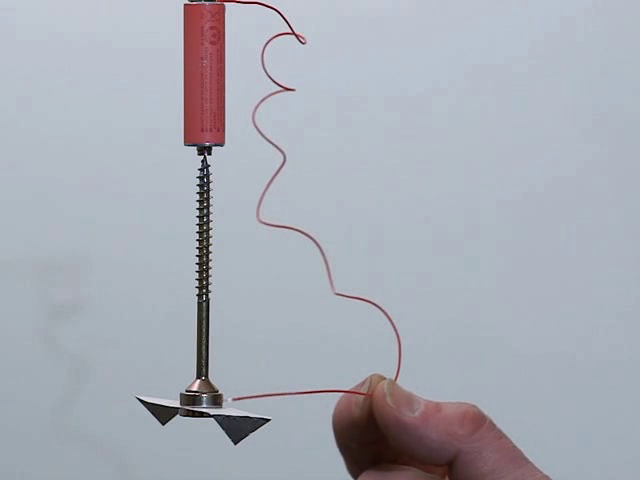
\includegraphics[height=0.4\textheight]{fig/lec03/homopolar_machine_video.png}}{fig/lec03/homopolar_machine_video.mp4}
            \vspace{0.75cm}
			\caption{Video of an operating homopolar machine (source: \href{https://de.wikipedia.org/wiki/Datei:Homopolarmotor_MAQ03891_smial_wp.ogv}{Wikimedia Commons}, Smial, \href{https://artlibre.org/licence/lal/en/}{Free Art License})}
		\end{subfigure}
		\hfill
		\begin{subfigure}[b]{0.49\textwidth}
			\centering
			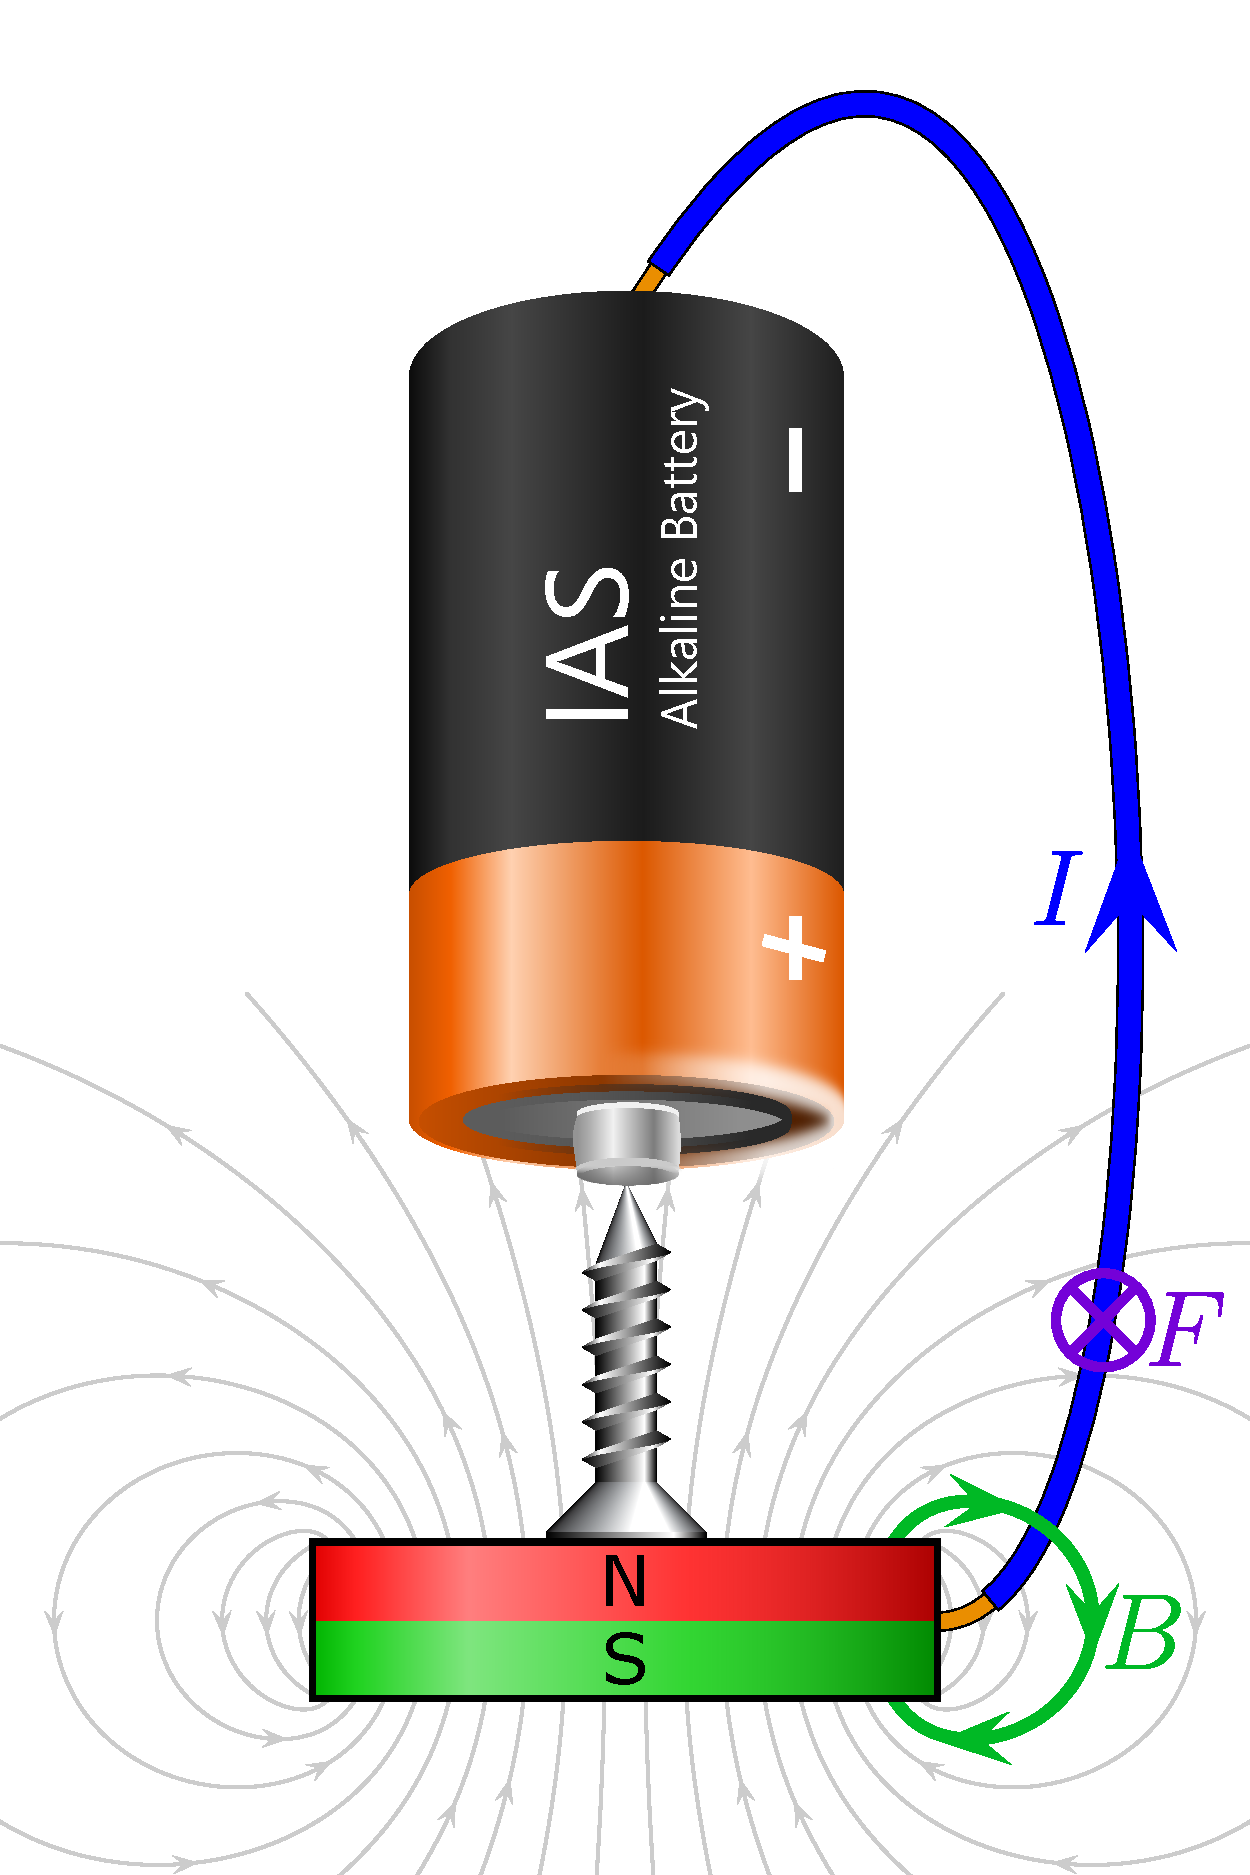
\includegraphics[width=0.47\textwidth]{fig/lec03/Homopolar_machine.pdf}
			\caption{Electric current, magnetic field and Lorentz force (adapted: \href{https://commons.wikimedia.org/wiki/File:Homopolar-motor.svg}{Wikimedia Commons}, M. Run, \href{https://creativecommons.org/licenses/by-sa/4.0/deed.en}{CC BY-SA})}
		\end{subfigure}
		\caption{Working principle of homopolar machines demonstrated with a simple permanent magnet, battery and screw design} 
        \label{fig:Homopolar_machine}
	\end{figure}
\end{frame}


%%%%%%%%%%%%%%%%%%%%%%%%%%%%%%%%%%%%%%%%%%%%%%%%%%%%%%%%%%%%%
%% Homopolar / unipolar machines (cont.) %%
%%%%%%%%%%%%%%%%%%%%%%%%%%%%%%%%%%%%%%%%%%%%%%%%%%%%%%%%%%%%%
\begin{frame}
	\frametitle{Homopolar / unipolar machines (cont.)}
    \begin{columns}
		\begin{column}{0.5\textwidth}
            \begin{itemize}
                \item  Homopolar machines are the simplest form of electric machines.
                \item They are also true DC machines, as the current and flux paths are unidirectional.
                \item<2-> The general design prevents connecting multiple rotor turns in series to increase the voltage, that is, only a relatively low voltage is induced.
                \item<3-> Consequently, homopolar machines require high currents (in the order of  \si{\kilo\ampere} or even \si{\mega\ampere}) to reach a useful power range which limited their application.
            \end{itemize}
		\end{column}
        \hfill
		\begin{column}{0.49\textwidth}
			\begin{figure}
				\centering
				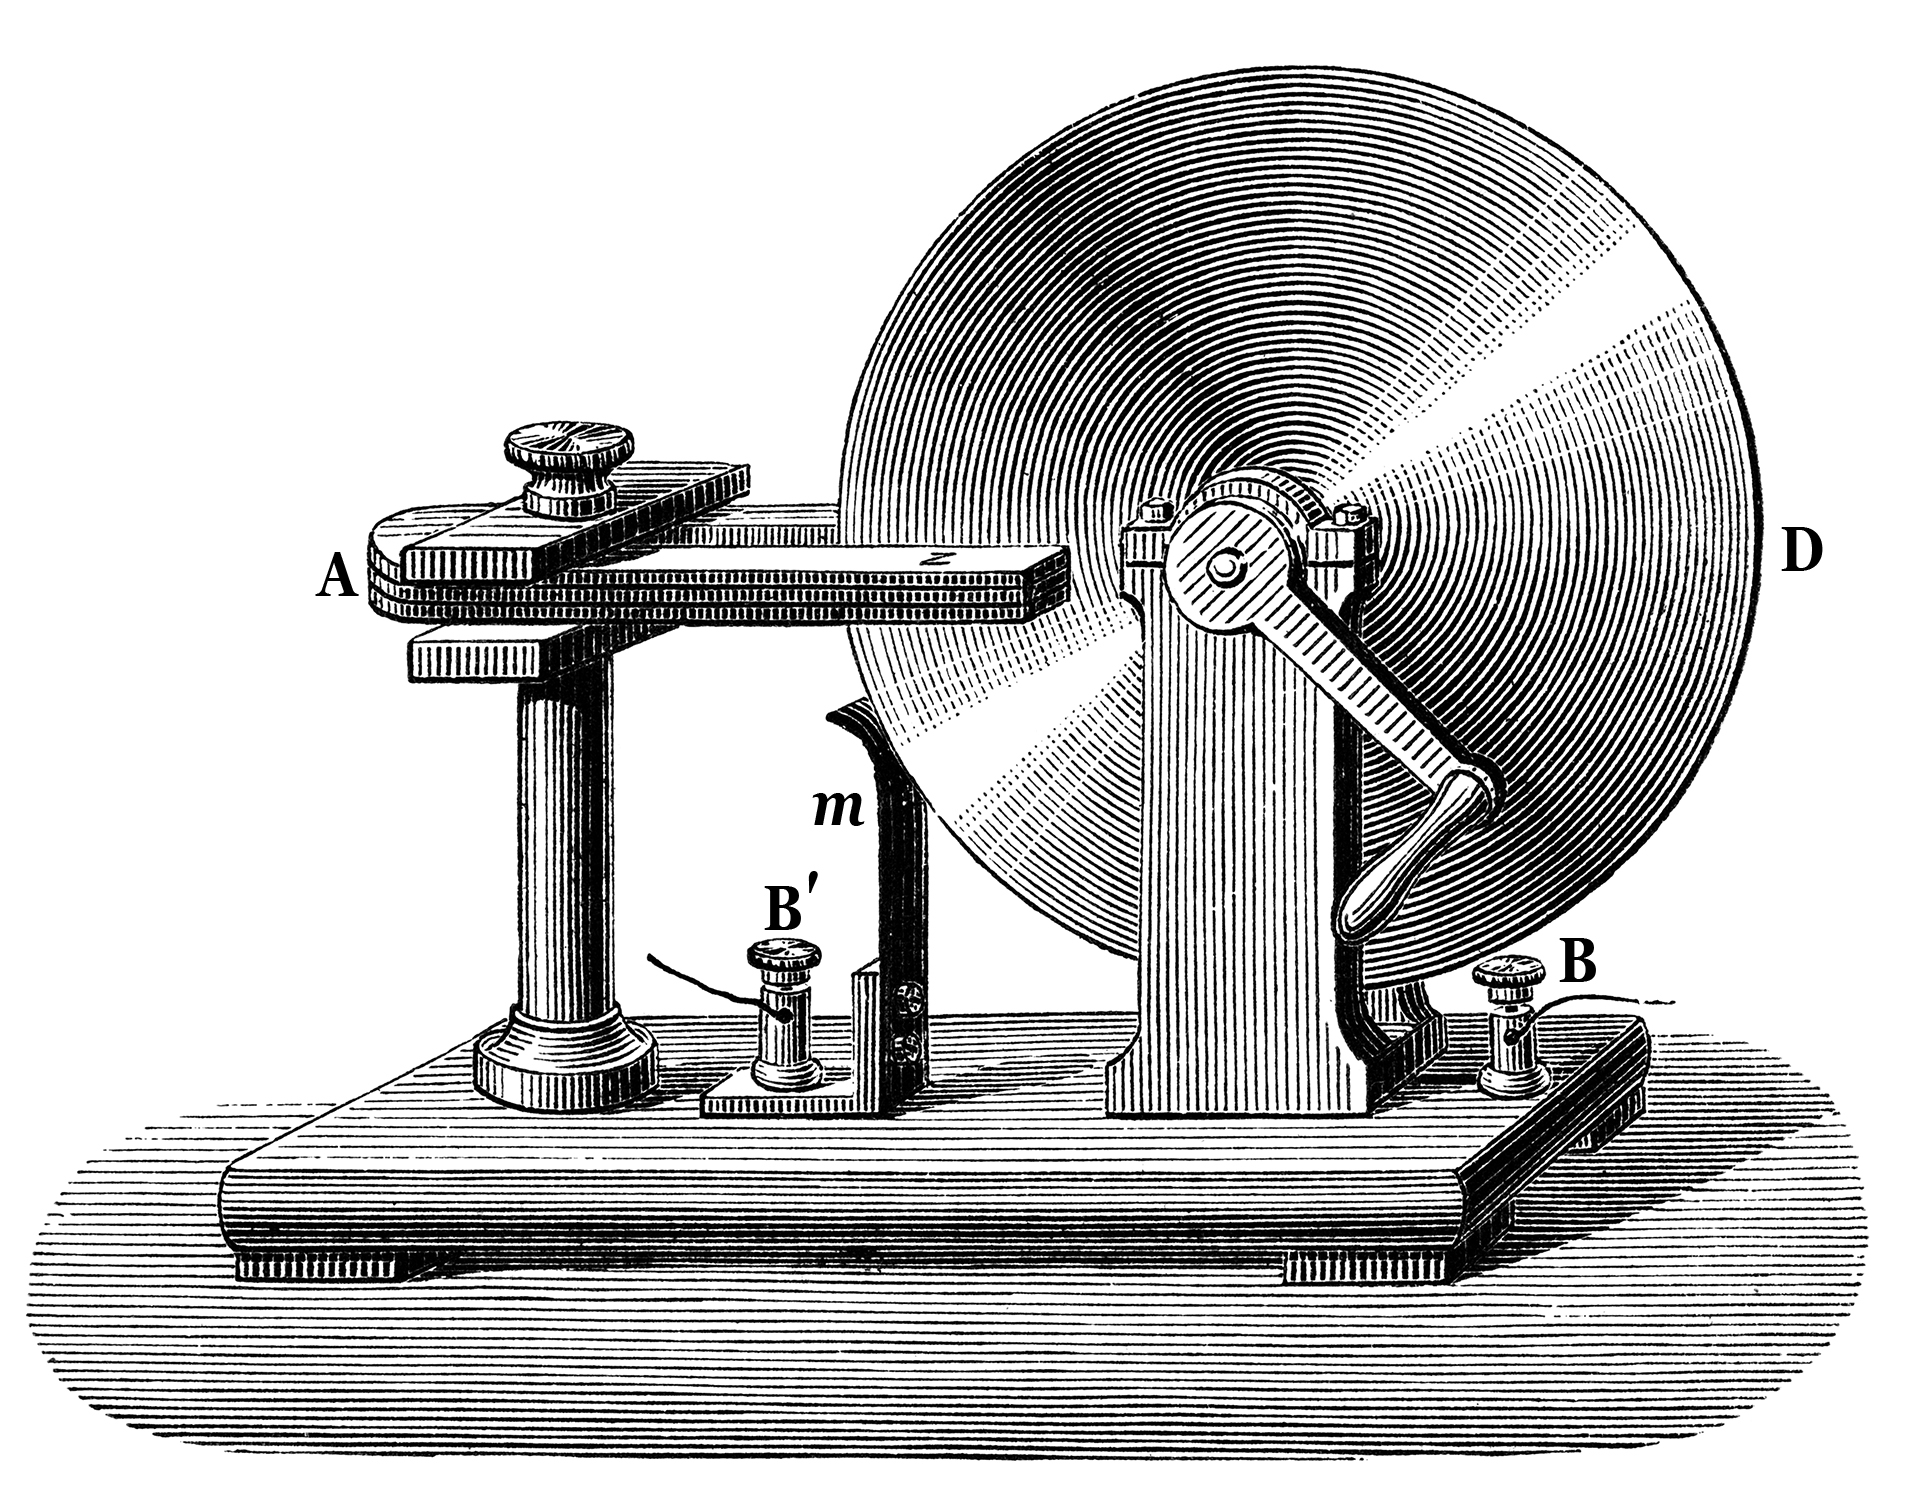
\includegraphics[width=0.8\textwidth]{fig/lec03/Faraday_disk_generator.jpg}
				\caption{The Faraday disk: another homopolar machine (source: \href{https://commons.wikimedia.org/wiki/File:Faraday_disk_generator.jpg}{Wikimedia Commons}, public domain)}
			\end{figure}
		\end{column}
		\end{columns}
\end{frame}

%%%%%%%%%%%%%%%%%%%%%%%%%%%%%%%%%%%%%%%%%%%%%%%%%%%%%%%%%%%%%
%% Working principle of usual DC machines %%
%%%%%%%%%%%%%%%%%%%%%%%%%%%%%%%%%%%%%%%%%%%%%%%%%%%%%%%%%%%%%
\begin{frame}
	\frametitle{Working principle of usual DC machines}
    \begin{columns}
		\begin{column}{0.5\textwidth}
            Let's consider \figref{fig:Simple_yoke_coil} and assume that the flux density $B$ is constant in the air gap and that the conductor loop has the axial length $l$. \onslide<2->{According to the Lorentz force we have
			\begin{equation}
				F = I_\mathrm{a} B l .
			\end{equation}}%  
			\onslide<3->{The torque $T$ on the conductor loop is given by
			\begin{equation}
				T = 2 F \frac{d}{2} \cos\left(\varepsilon\right) = I_\mathrm{a} B l d \cos\left(\varepsilon\right).
			\end{equation}}%
			\onslide<4->{If the loop spins with an angular velocity $\omega$, mechanical power $P_\mathrm{me} = T\omega$ is transferred. 
			\\[1em]}%
			\onslide<5->{\textbf{Question:} What is happening if the coil is outside the magnetic field?}
		\end{column}
        \hfill
		\begin{column}{0.49\textwidth}
			\begin{figure}
				\centering
				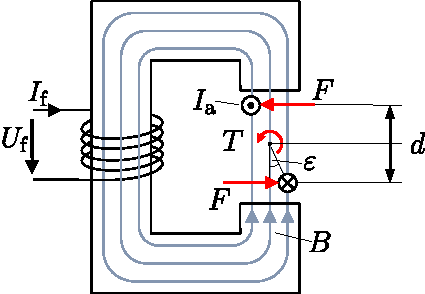
\includegraphics[width=0.9\textwidth]{fig/lec03/Simple_yoke_coil.pdf}
				\caption{Torque on a conductor loop (adapted from J.~B\"ocker, \textit{Elektrische Antriebstechnik}, Paderborn University, 2020)}
				\label{fig:Simple_yoke_coil}
			\end{figure}
		\end{column}
		\end{columns}
\end{frame}

%%%%%%%%%%%%%%%%%%%%%%%%%%%%%%%%%%%%%%%%%%%%%%%%%%%%%%%%%%%%%
%% DC-machine cross section %%
%%%%%%%%%%%%%%%%%%%%%%%%%%%%%%%%%%%%%%%%%%%%%%%%%%%%%%%%%%%%%
\begin{frame}
	\frametitle{DC-machine cross section}
    \begin{columns}
		\begin{column}{0.42\textwidth}
            \begin{itemize}
				\item To ensure a quasi-continous torque, the current through the conductor loop(s) in the rotor must have a constant direction.
				\item<2-> This is achieved by using a commutator (brushes).
				\item<3-> Compared to homopolar machines, DC machines require a mechanical rectification of the current.
			\end{itemize}
		\end{column}
        \hfill
		\begin{column}{0.55\textwidth}
			\begin{figure}
				\centering
				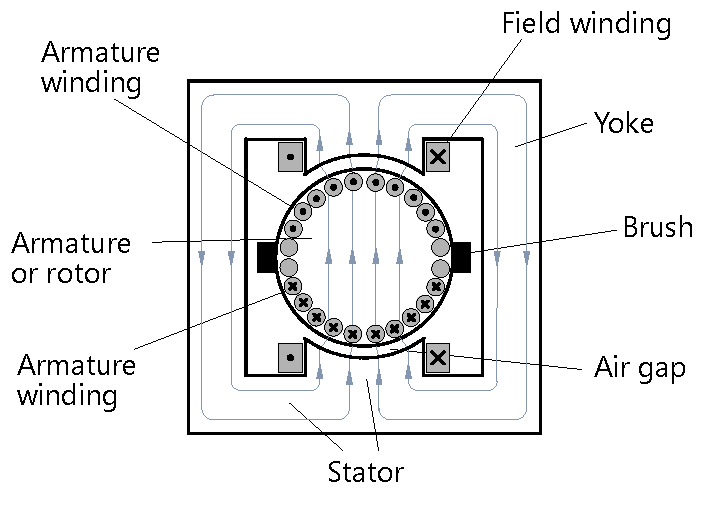
\includegraphics[width=0.925\textwidth]{fig/lec03/DC_machine_cross_section.pdf}
				\caption{Simplified DC machine cross section (adapted from J.~B\"ocker, \textit{Elektrische Antriebstechnik}, Paderborn University, 2020)}
				\label{fig:DC_machine_cross_section}
			\end{figure}
		\end{column}
		\end{columns}
\end{frame}

%%%%%%%%%%%%%%%%%%%%%%%%%%%%%%%%%%%%%%%%%%%%%%%%%%%%%%%%%%%%%
%% Commutation %%
%%%%%%%%%%%%%%%%%%%%%%%%%%%%%%%%%%%%%%%%%%%%%%%%%%%%%%%%%%%%%
\begin{frame}
	\frametitle{Commutation}
    \begin{figure}
		\centering
		\movie{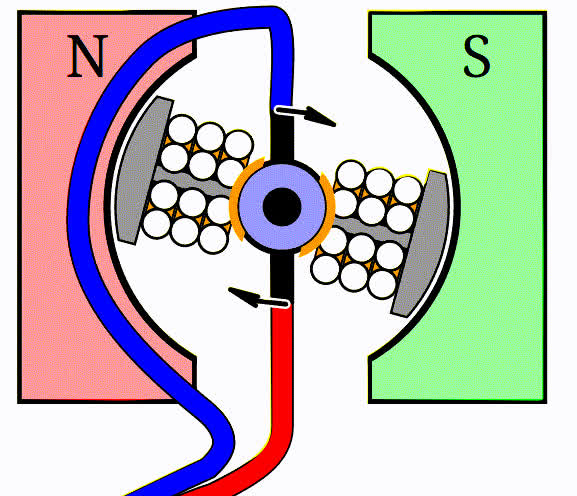
\includegraphics[height=0.65\textheight]{fig/lec03/DC_machine_simple_animation.jpeg}}{fig/lec03/DC_machine_simple_animation.gif}
		\caption{Animation of the commutation process \\(source: \href{https://commons.wikimedia.org/wiki/File:Animation_einer_Gleichstrommaschine_(Variante-Langsam).gif}{Wikimedia Commons}, M. Frey, \href{https://creativecommons.org/licenses/by-sa/3.0/deed.en}{CC BY-SA 3.0})}
	\end{figure}
\end{frame}

%%%%%%%%%%%%%%%%%%%%%%%%%%%%%%%%%%%%%%%%%%%%%%%%%%%%%%%%%%%%%
%% Armature and commutator %%
%%%%%%%%%%%%%%%%%%%%%%%%%%%%%%%%%%%%%%%%%%%%%%%%%%%%%%%%%%%%%
\begin{frame}
	\frametitle{Armature and commutator}
    \begin{figure}
		\centering
		\begin{subfigure}[b]{0.49\textwidth}
			\centering
			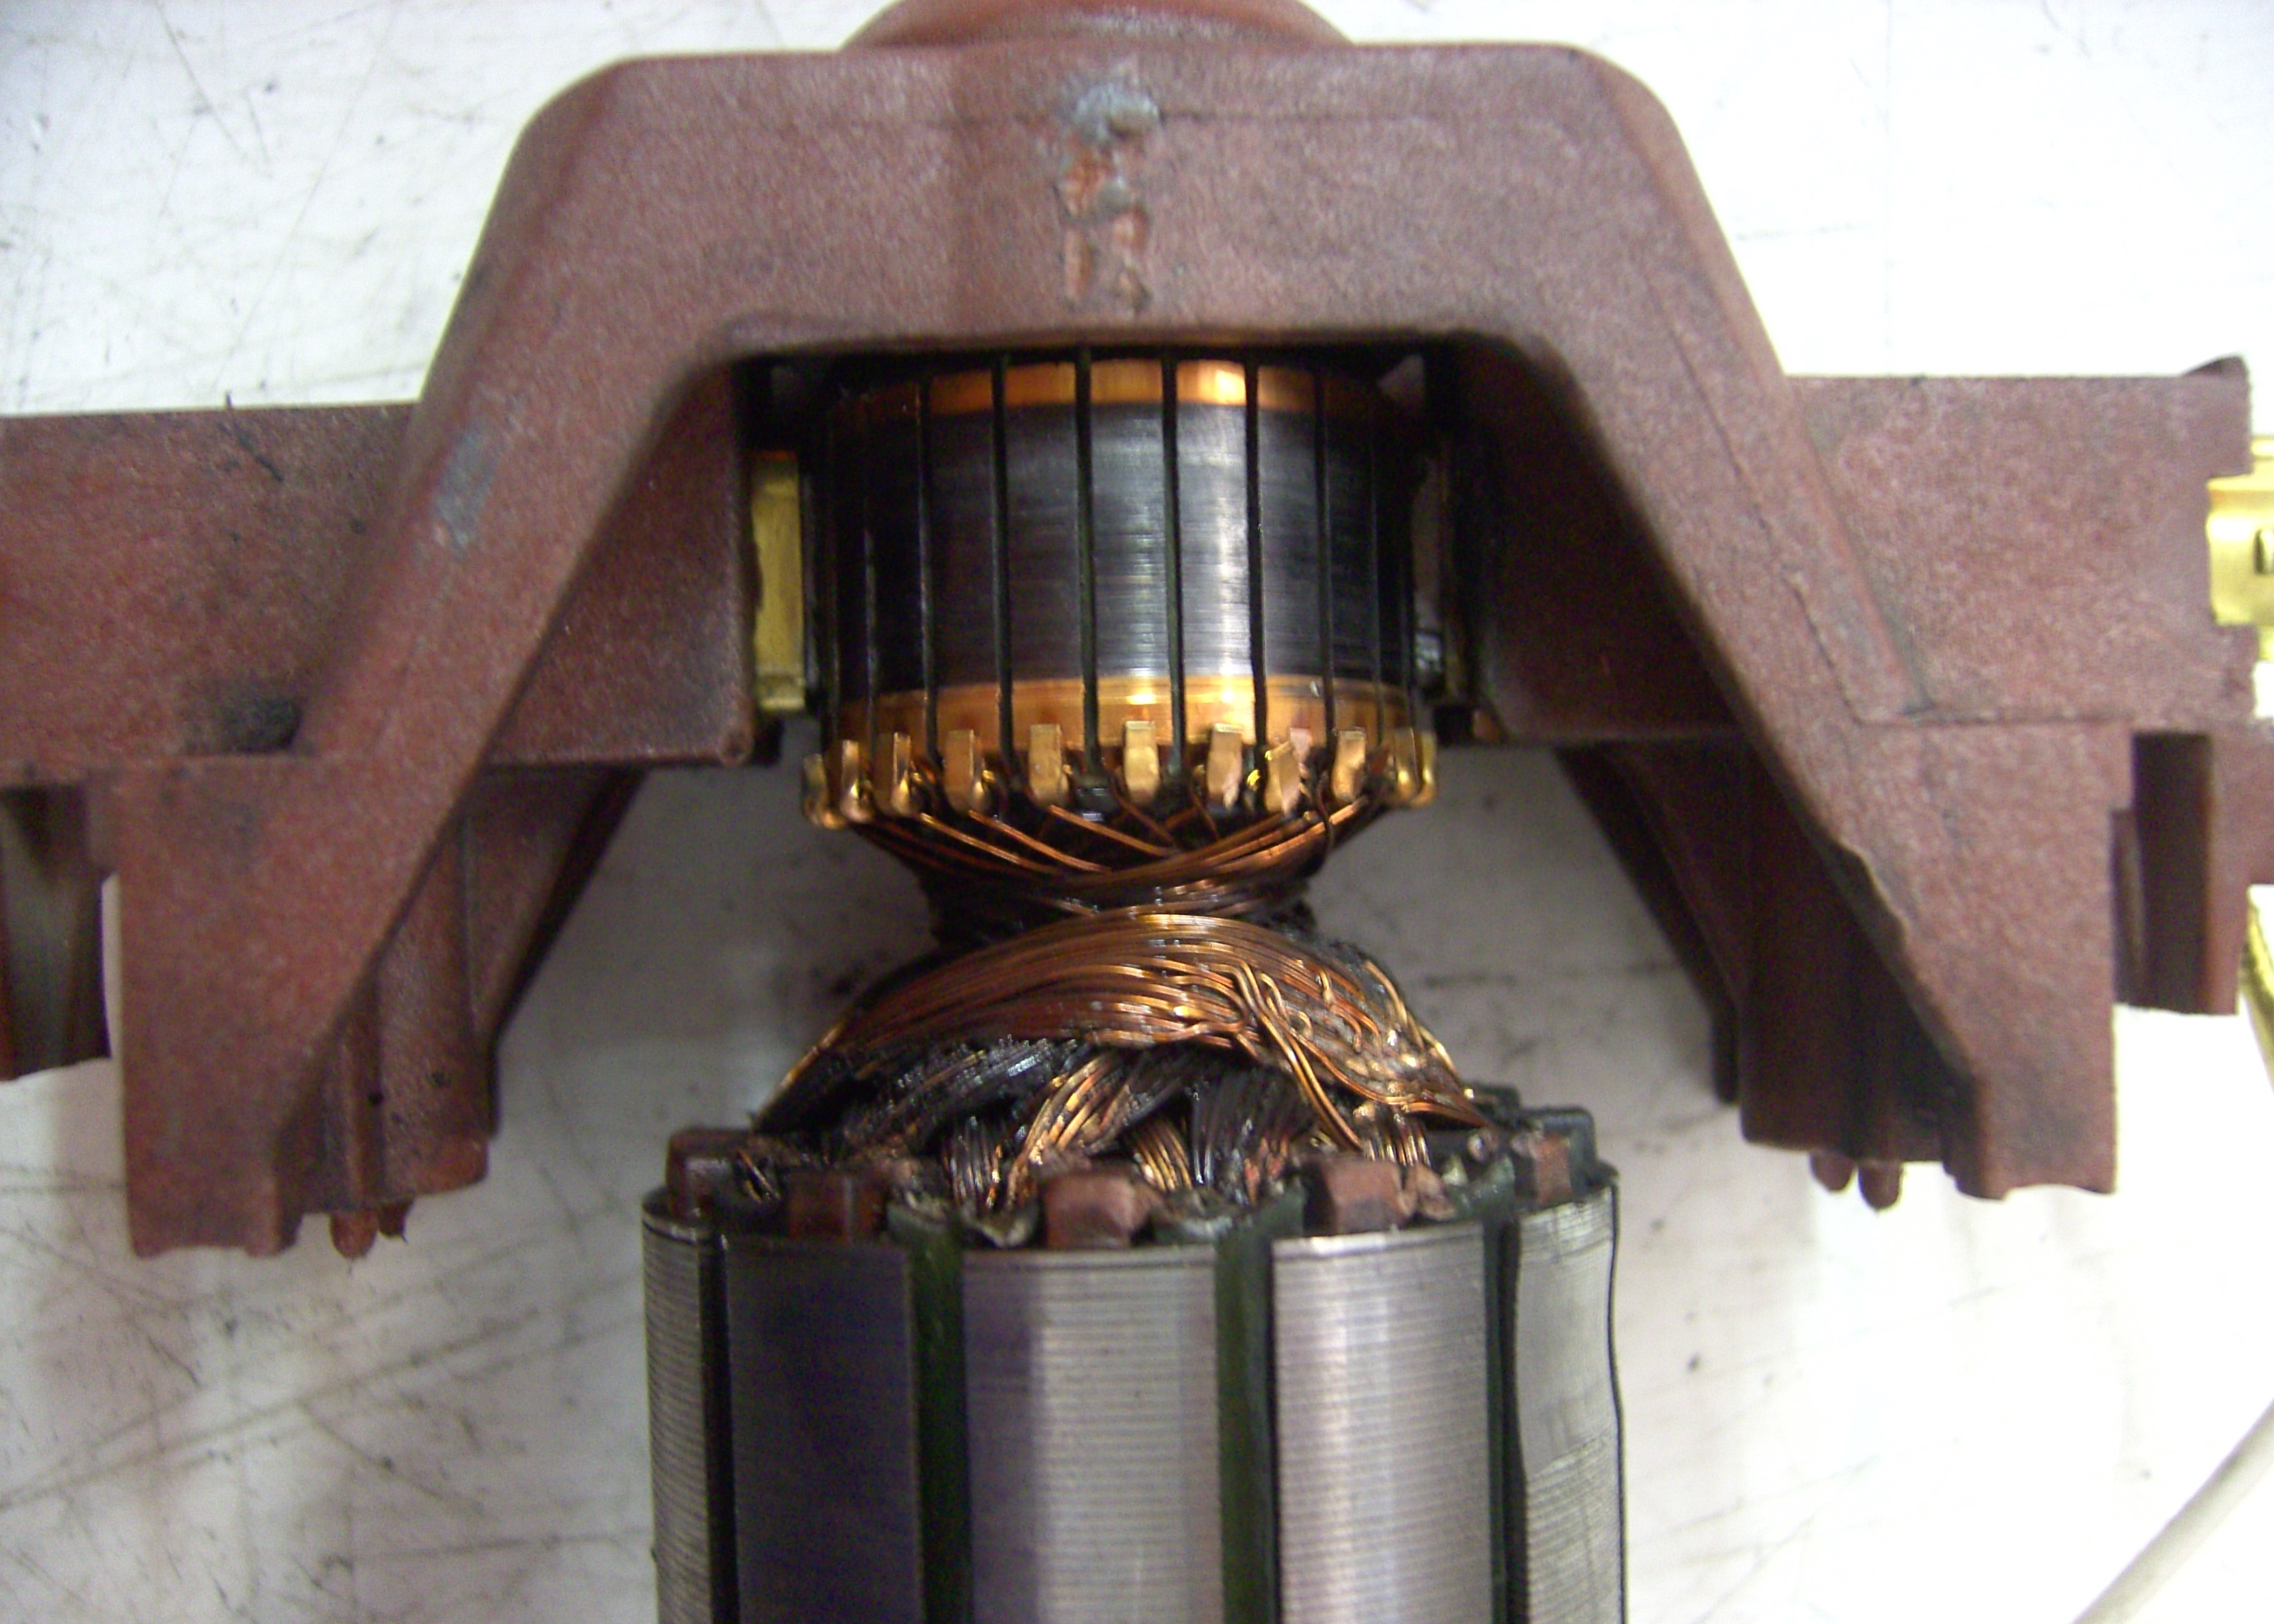
\includegraphics[width=0.85\textwidth]{fig/lec03/Commutator_Universalmachine.jpg}
			\caption{Commutator with brushes and springs (source: \href{https://commons.wikimedia.org/wiki/File:Kommutator_eines_Universalmotor.JPGg}{Wikimedia Commons}, Marrrci, \href{https://creativecommons.org/licenses/by-sa/3.0/deed.en}{CC BY-SA 3.0})}
		\end{subfigure}
		\hfill
		\begin{subfigure}[b]{0.49\textwidth}
			\centering
			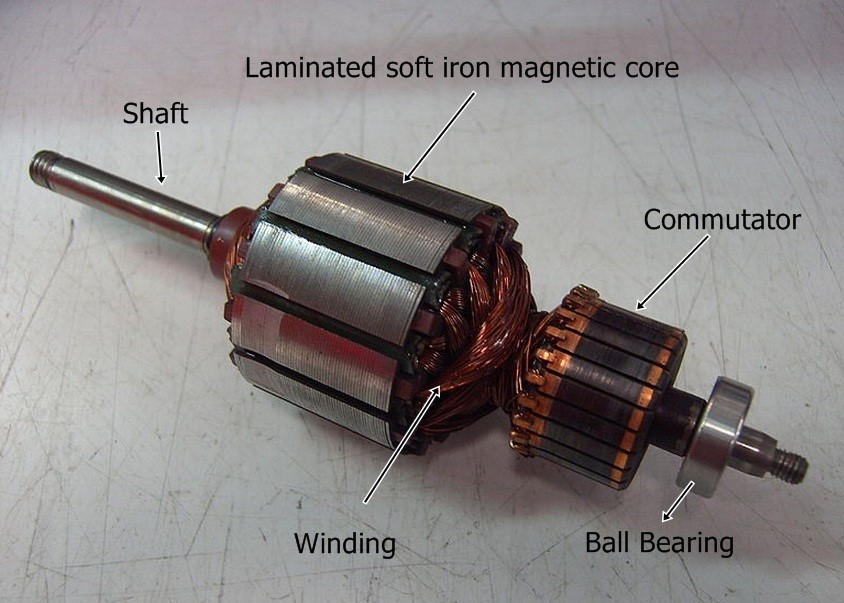
\includegraphics[width=0.85\textwidth]{fig/lec03/DC_armature_example.jpg}
			\caption{DC machine armature with commutator (source: \href{https://commons.wikimedia.org/wiki/File:Motor_rotor.jpg}{Wikimedia Commons}, public domain)}
		\end{subfigure}
		\caption{Examples of commutators and armatures} 
        \label{fig:Armature_and_commutator}
	\end{figure}
\end{frame}

%%%%%%%%%%%%%%%%%%%%%%%%%%%%%%%%%%%%%%%%%%%%%%%%%%%%%%%%%%%%%
%% Armature and commutator (cont.) %%
%%%%%%%%%%%%%%%%%%%%%%%%%%%%%%%%%%%%%%%%%%%%%%%%%%%%%%%%%%%%%
\begin{frame}
	\frametitle{Armature and commutator (cont.)}
    \begin{figure}
		\centering
		\begin{subfigure}[b]{0.49\textwidth}
			\centering
			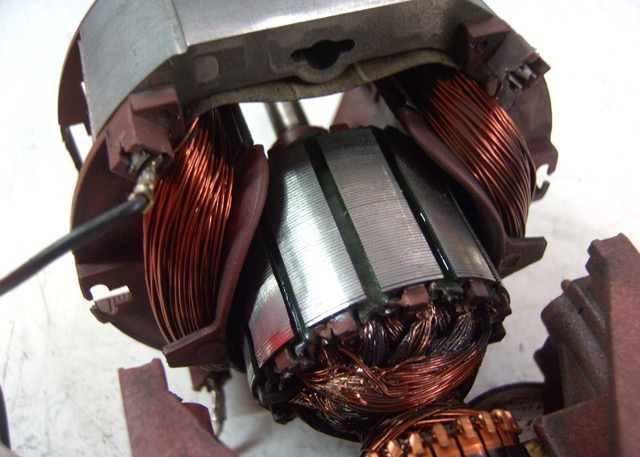
\includegraphics[width=0.85\textwidth]{fig/lec03/Stator_Rotor_Universalmachine.jpg}
			\caption{Armature inside stator (source: \href{https://commons.wikimedia.org/wiki/File:Universalmotor_1.JPG}{Wikimedia Commons}, Marrrci, \href{https://creativecommons.org/licenses/by-sa/3.0/deed.en}{CC BY-SA 3.0})}
		\end{subfigure}
		\hfill
		\begin{subfigure}[b]{0.49\textwidth}
			\centering
			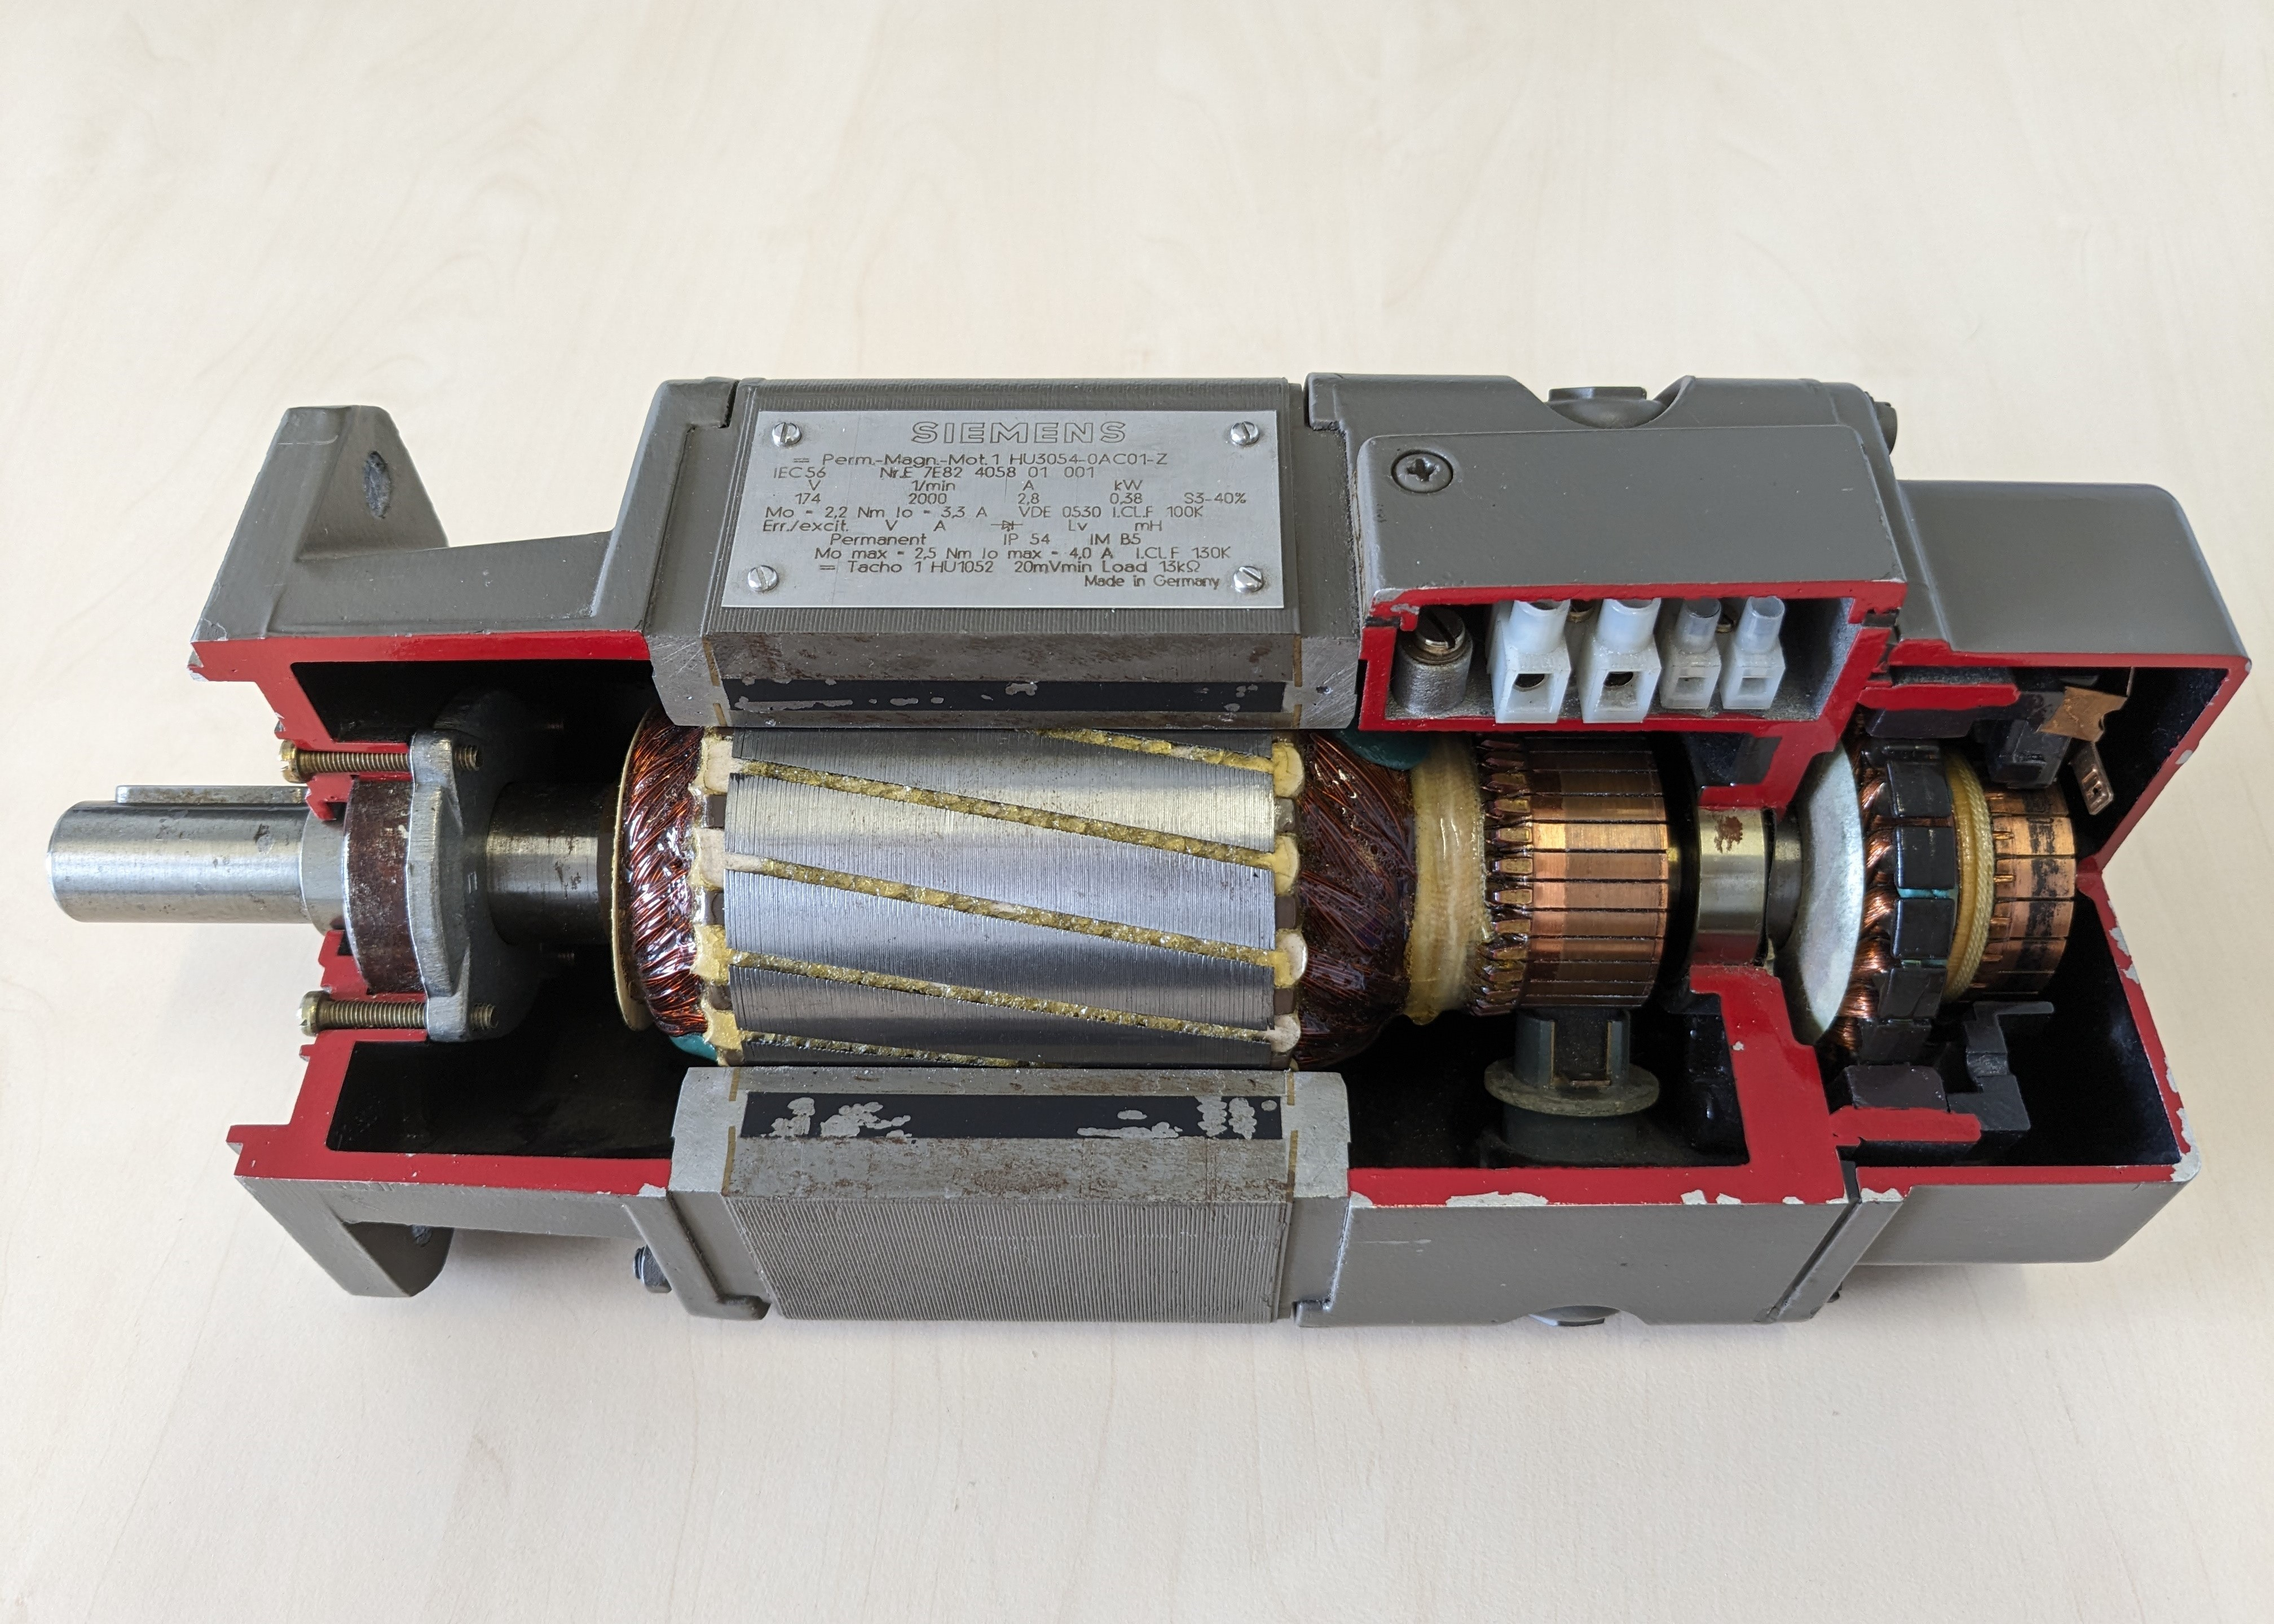
\includegraphics[width=0.85\textwidth]{fig/lec03/DC_Machine_PM.jpg}
			\caption{DC machine with permanent magnet excitation and tacho speed sensor}
		\end{subfigure}
		\caption{Examples of commutators and armatures (cont.)} 
        \label{fig:Armature_and_commutator_02}
	\end{figure}
\end{frame}

%%%%%%%%%%%%%%%%%%%%%%%%%%%%%%%%%%%%%%%%%%%%%%%%%%%%%%%%%%%%%
%% Basic structure of the armature %%
%%%%%%%%%%%%%%%%%%%%%%%%%%%%%%%%%%%%%%%%%%%%%%%%%%%%%%%%%%%%%
\begin{frame}
	\frametitle{Basic structure of the armature}
    \begin{figure}
        \centering
        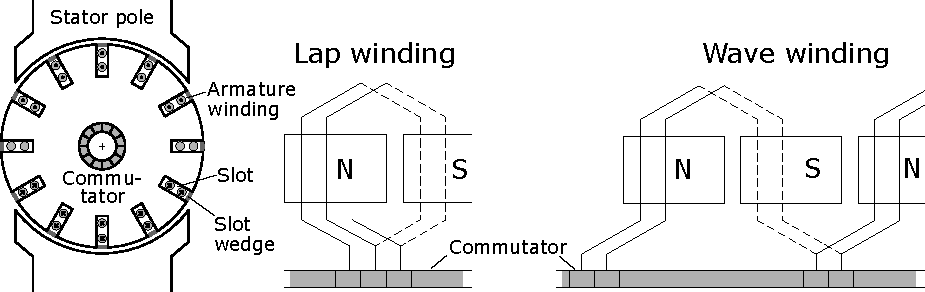
\includegraphics[width=0.925\textwidth]{fig/lec03/Armature_slots.pdf}
        \caption{Cross section of a drum-type armature including principle winding schemes (adapted from W.~Novender, \textit{Elektrische Maschinen}, Technische Hochschule Mittelhessen, 2023)}
    \end{figure}
\end{frame}

%%%%%%%%%%%%%%%%%%%%%%%%%%%%%%%%%%%%%%%%%%%%%%%%%%%%%%%%%%%%%
%% Commutation process with an armature lap winding %%
%%%%%%%%%%%%%%%%%%%%%%%%%%%%%%%%%%%%%%%%%%%%%%%%%%%%%%%%%%%%%
\begin{frame}
	\frametitle{Commutation process with an armature lap winding}
	\vspace{-0.1cm}
    \begin{figure}
        \centering
        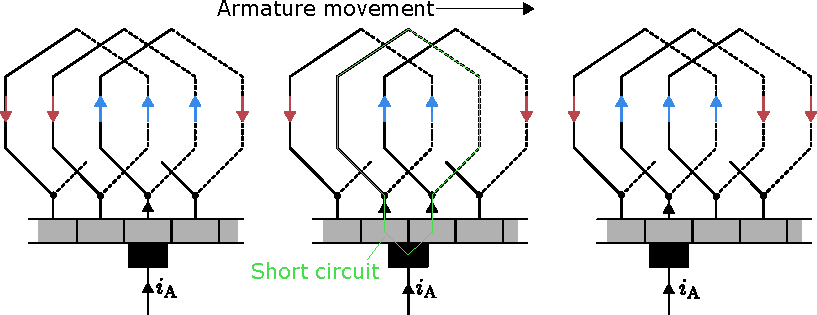
\includegraphics[height=0.6\textheight]{fig/lec03/Commutation_process_lap_winding.pdf}
        \caption{Three still images of the commutation process with a simplified winding representation (from left to right): when the brush touches two commutator segments, the according conductor loop is short-circuited and the current is reduced to zero. The brush then moves to the next commutator segment and the current starts flowing again but in the opposite direction (adapted from W.~Novender, \textit{Elektrische Maschinen}, Technische Hochschule Mittelhessen, 2023).}
    \end{figure}
\end{frame}

%%%%%%%%%%%%%%%%%%%%%%%%%%%%%%%%%%%%%%%%%%%%%%%%%%%%%%%%%%%%%
%% DC machines with multiple pole pairs %%
%%%%%%%%%%%%%%%%%%%%%%%%%%%%%%%%%%%%%%%%%%%%%%%%%%%%%%%%%%%%%
\begin{frame}
	\frametitle{DC machines with multiple pole pairs}
    \begin{columns}
		\begin{column}{0.42\textwidth}
            \begin{itemize}
				\item To reduce the effective length per armature conductor loop, the winding can form multiple pole pairs $p$.
				\item<2-> This will reduce the inductance per loop which is beneficial for the commutation process.
				\item<3-> The stator excitation must meet the same number of pole pairs.
				\item<4-> Given some inner stator diameter $d_\mathrm{s}$, the resulting pole pitch is:
			\end{itemize}
			\onslide<4->{\begin{equation}
				\tau_\mathrm{p} = \frac{\pi d_\mathrm{s}}{2p}, \quad \rho_\mathrm{p} = \frac{\pi}{p} .
			\end{equation}}%
		\end{column}
        \hfill
		\begin{column}{0.55\textwidth}
			\begin{figure}
				\centering
				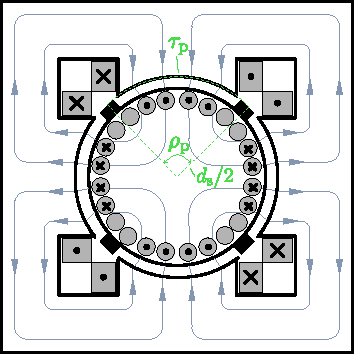
\includegraphics[width=0.64\textwidth]{fig/lec03/DC_machine_cross_section_two_pole_pairs.pdf}
				\caption{Simplified DC machine cross section with $p=2$ pole pairs (adapted from J.~B\"ocker, \textit{Elektrische Antriebstechnik}, Paderborn University, 2020)}
			\end{figure}
		\end{column}
		\end{columns}
\end{frame}

%%%%%%%%%%%%%%%%%%%%%%%%%%%%%%%%%%%%%%%%%%%%%%%%%%%%%%%%%%%%%
%% Winding characteristics (cont.) %%
%%%%%%%%%%%%%%%%%%%%%%%%%%%%%%%%%%%%%%%%%%%%%%%%%%%%%%%%%%%%%
\begin{frame}
	\frametitle{Armature winding characteristics}
	For describing the armature winding layout, the following parameters are introduced:
	\begin{gather*}
		Q: \mbox{number of slots}, \quad N_\mathrm{c}: \mbox{number of conductor turns per coil}, \\ K: \mbox{number of commutator elements}, \quad u = K/Q: \mbox{slot to commutator ratio}, \\z_\mathrm{a} = 2 K N_\mathrm{c}: \mbox{total number of armature conductors}.
	\end{gather*}
    \begin{figure}
        \centering
        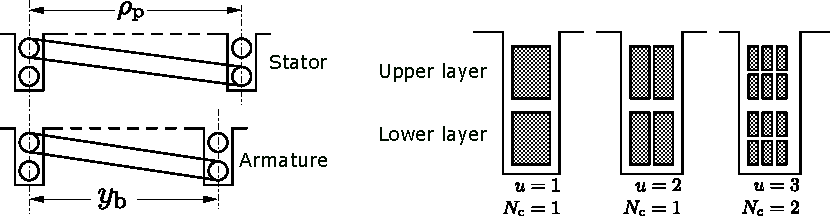
\includegraphics[height=0.35\textheight]{fig/lec03/Lap_winding_characteristics.pdf}
        \caption{Coil width and slot design characteristics (adapted from W.~Novender, \textit{Elektrische Maschinen}, Technische Hochschule Mittelhessen, 2023)}
		\label{fig:Lap_winding_characteristics}
    \end{figure}
\end{frame}

%%%%%%%%%%%%%%%%%%%%%%%%%%%%%%%%%%%%%%%%%%%%%%%%%%%%%%%%%%%%%
%% Double layer winding %%
%%%%%%%%%%%%%%%%%%%%%%%%%%%%%%%%%%%%%%%%%%%%%%%%%%%%%%%%%%%%%
\begin{frame}
	\frametitle{Double layer winding}
	\begin{itemize}
		\item The forward conductor of one coil and the return conductor of another coil are placed in the same slot. This is the common winding scheme (although not limited to it).
		\item Enables chording of the winding ($\rho_\mathrm{p}\neq y_\mathrm{b}$), another degree of freedom for the machine design (cf. \figref{fig:Lap_winding_characteristics}).
	\end{itemize}
    \begin{figure}
        \centering
        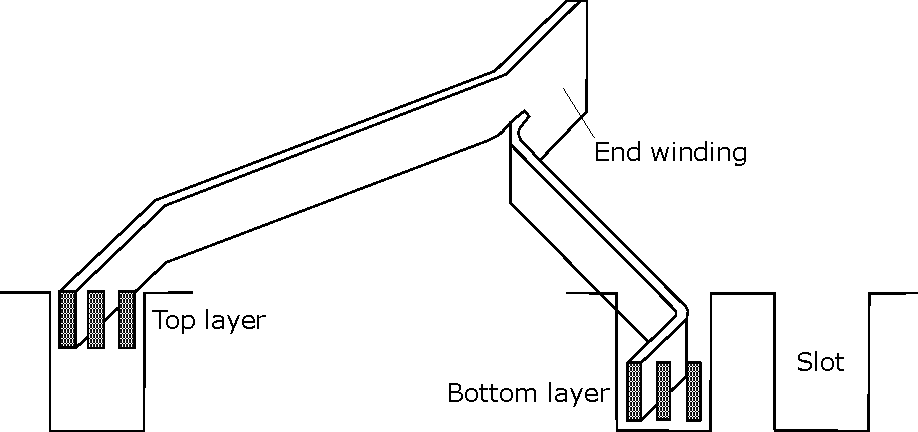
\includegraphics[height=0.45\textheight]{fig/lec03/Double_layer_winding.pdf}
        \caption{Double layer winding with $u=3$ with a solid conductor element (which can be pre-manufactured for cost reasons -- inspired from A. Binder, \textit{Elektrische Maschinen und Antriebe}, Vol. 2, Springer, 2017)}
    \end{figure}
\end{frame}

%%%%%%%%%%%%%%%%%%%%%%%%%%%%%%%%%%%%%%%%%%%%%%%%%%%%%%%%%%%%%
%% Lap winding characteristics %%
%%%%%%%%%%%%%%%%%%%%%%%%%%%%%%%%%%%%%%%%%%%%%%%%%%%%%%%%%%%%%
\begin{frame}
	\frametitle{Lap winding characteristics}
    \begin{columns}
		\begin{column}{0.42\textwidth}
            \begin{itemize}
				\item Back pitch $y_\mathrm{b}$: coil span from the back end
				\item<2-> Front pitch $y_\mathrm{f}$: coil span from the front end
				\item<3-> Resultant pitch $y_\mathrm{r}$: distance between two consecutive coils
				\item<4-> Commutator pitch $y_\mathrm{c}$: distance between two consecutive commutator segments
			\end{itemize}
			\vspace{-0.4cm}
			\onslide<5->{\begin{varblock}{Progressive winding}
				\figref{fig:Lap_winding_distances} shows a progressive winding layout with $y_\mathrm{b} > y_\mathrm{f}$, i.e., the coils do not cross themselves.
			\end{varblock}}%
		\end{column}
        \hfill
		\begin{column}{0.55\textwidth}
			\begin{figure}
				\centering
				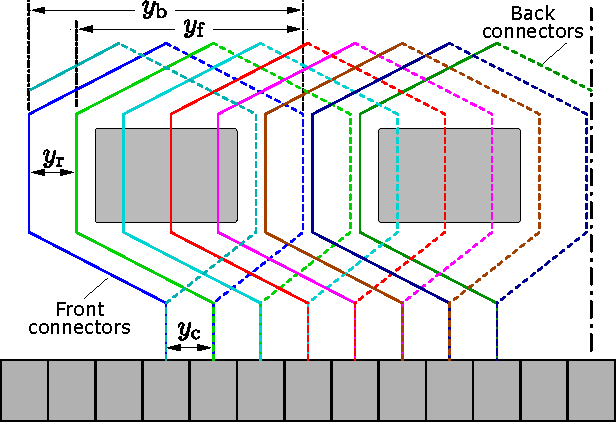
\includegraphics[width=0.85\textwidth]{fig/lec03/Lap_winding_distances.pdf}
				\caption{Distance definitions of the armature lap winding (adapted from W.~Novender, \textit{Elektrische Maschinen}, Technische Hochschule Mittelhessen, 2023)}
				\label{fig:Lap_winding_distances}
			\end{figure}
		\end{column}
		\end{columns}
\end{frame}

%%%%%%%%%%%%%%%%%%%%%%%%%%%%%%%%%%%%%%%%%%%%%%%%%%%%%%%%%%%%%
%% Lap winding characteristics (cont.) %%
%%%%%%%%%%%%%%%%%%%%%%%%%%%%%%%%%%%%%%%%%%%%%%%%%%%%%%%%%%%%%
\begin{frame}
	\frametitle{Lap winding characteristics (cont.)}
    \begin{columns}
		\begin{column}{0.42\textwidth}
			\begin{varblock}{Retrogressive winding}
				\figref{fig:Lap_winding_distances_retrogressive} shows a Retrogressive winding layout with $y_\mathrm{b} < y_\mathrm{f}$, i.e., each coil crosses itself.
			\end{varblock}
			\begin{itemize}
				\item<2-> Retrogressive windings require more conductor material due to the crossing of the coils and, therefore, are less common.
				\item<3-> Technical feasibility requires $y_\mathrm{b} - y_\mathrm{f} = \pm y_\mathrm{c}$, i.e., the lap winding progresses or retrogresses by one commutator element.
			\end{itemize}
		\end{column}
        \hfill
		\begin{column}{0.55\textwidth}
			\begin{figure}
				\centering
				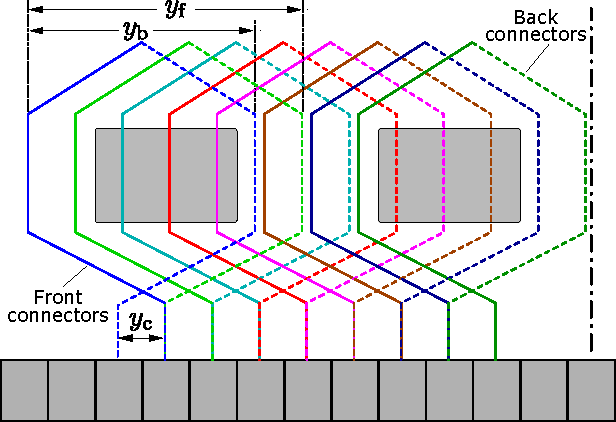
\includegraphics[width=0.85\textwidth]{fig/lec03/Lap_winding_distances_retrogressive.pdf}
				\caption{Lap winding with a retrogressive scheme (adapted from W.~Novender, \textit{Elektrische Maschinen}, Technische Hochschule Mittelhessen, 2023)}
				\label{fig:Lap_winding_distances_retrogressive}
			\end{figure}
		\end{column}
		\end{columns}
\end{frame}


%%%%%%%%%%%%%%%%%%%%%%%%%%%%%%%%%%%%%%%%%%%%%%%%%%%%%%%%%%%%%
%% Lap winding %%
%%%%%%%%%%%%%%%%%%%%%%%%%%%%%%%%%%%%%%%%%%%%%%%%%%%%%%%%%%%%%
\begin{frame}
	\frametitle{Lap winding: final remarks and single pole pair example}
	\begin{columns}
		\begin{column}{0.35\textwidth}
			\begin{itemize}
				\item Armature turns per pole: $N_\mathrm{p} = \frac{KN_\mathrm{c}}{2p}$
				\item Current per armature conductor: $I_\mathrm{c} = \frac{I_\mathrm{a}}{2 p}$
			\end{itemize}
			\onslide<2->{\begin{varblock}{Parallel connection of poles}
				For $p>1$ the lap winding parallels the armature coils for each pole enabling a higher current (but limited voltage) rating.
			\end{varblock}}%
		\end{column}
		\hfill
		\begin{column}{0.65\textwidth}
			\begin{figure}
				\centering
				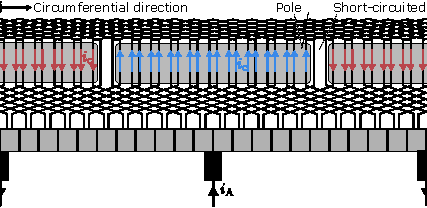
\includegraphics[width=0.95\textwidth]{fig/lec03/Lap_winding.pdf}
				\caption{Lap winding with commutator unrolled along the circumferential coordinate}
			\end{figure}
		\end{column}
	\end{columns}
\end{frame}

%%%%%%%%%%%%%%%%%%%%%%%%%%%%%%%%%%%%%%%%%%%%%%%%%%%%%%%%%%%%%
%% Wave winding characteristics %%
%%%%%%%%%%%%%%%%%%%%%%%%%%%%%%%%%%%%%%%%%%%%%%%%%%%%%%%%%%%%%
\begin{frame}
	\frametitle{Wave winding characteristics}
    \begin{columns}
		\begin{column}{0.42\textwidth}
            \begin{itemize}
				\item Commutator pitch (wave winding): $y_\mathrm{c} = y_\mathrm{f} + y_\mathrm{b}$, i.e., each coil spans (nearly) the entire pole pitch.  
			\end{itemize}
			\vspace{-0.4cm}
			\onslide<2->{\begin{varblock}{Progressive winding}
				\figref{fig:Wave_winding_distances} shows a progressive winding layout since each new wave winding coil starts one commutator element to the right. 
			\end{varblock}}"
		\end{column}
        \hfill
		\begin{column}{0.55\textwidth}
			\begin{figure}
				\centering
				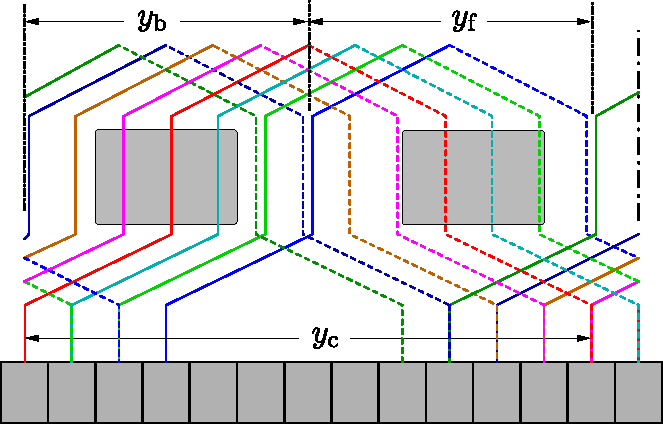
\includegraphics[width=0.85\textwidth]{fig/lec03/Wave_winding_distances.pdf}
				\caption{Distance definitions of the armature wave winding (adapted from W.~Novender, \textit{Elektrische Maschinen}, Technische Hochschule Mittelhessen, 2023)}
				\label{fig:Wave_winding_distances}
			\end{figure}
		\end{column}
		\end{columns}
\end{frame}

%%%%%%%%%%%%%%%%%%%%%%%%%%%%%%%%%%%%%%%%%%%%%%%%%%%%%%%%%%%%%
%% Wave winding %%
%%%%%%%%%%%%%%%%%%%%%%%%%%%%%%%%%%%%%%%%%%%%%%%%%%%%%%%%%%%%%
\begin{frame}
	\frametitle{Wave winding: final remarks and single pole pair example}
	\begin{columns}
		\begin{column}{0.35\textwidth}
			\begin{itemize}
				\item Armature turns per pole: $N_\mathrm{p} = \frac{K N_\mathrm{c}}{2}$
				\item Current per armature conductor: $I_\mathrm{c} = \frac{I_\mathrm{a}}{2}$
			\end{itemize}
			\onslide<2->{\begin{varblock}{Series connection of poles}
				For $p>1$ the wave winding connects the armature coils for all poles in series enabling a higher voltage (but limited current) rating.
			\end{varblock}}
		\end{column}
		\hfill
		\begin{column}{0.65\textwidth}
			\begin{figure}
				\centering
				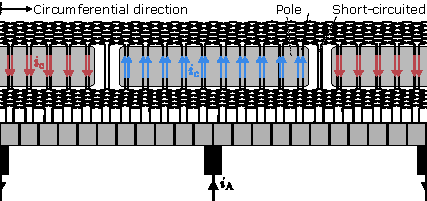
\includegraphics[width=0.95\textwidth]{fig/lec03/Wave_winding.pdf}
				\caption{Wave winding with commutator unrolled along the circumferential coordinate}
			\end{figure}
		\end{column}
	\end{columns}
\end{frame}

%%%%%%%%%%%%%%%%%%%%%%%%%%%%%%%%%%%%%%%%%%%%%%%%%%%%%%%%%%%%%
%% Lap and wave winding comparison %%
%%%%%%%%%%%%%%%%%%%%%%%%%%%%%%%%%%%%%%%%%%%%%%%%%%%%%%%%%%%%%
\begin{frame}
	\frametitle{Lap and wave winding comparison}
	Introducing the parameter 
	\begin{equation}
		a = \mbox{Number of parallel armature conductors}
	\end{equation}
	we can wrap up the following summary:\pause
	\begin{equation}
		\mbox{Current per conductor: } I_\mathrm{c} = \frac{I_\mathrm{a}}{2 a}, \quad \mbox{Armature turns per pole: } N_\mathrm{p} = \frac{K N_\mathrm{c}}{2 a}.
	\end{equation}\pause
	\begin{varblock}{Comparison}
		\begin{itemize}
			\item Lap winding: $a = p$ (parallel connection of poles)
			\item Wave winding: $a = 1$ (series connection of poles)
		\end{itemize}
	\end{varblock}

\end{frame}

%%%%%%%%%%%%%%%%%%%%%%%%%%%%%%%%%%%%%%%%%%%%%%%%%%%%%%%%%%%%%
%% Air gap field %%
%%%%%%%%%%%%%%%%%%%%%%%%%%%%%%%%%%%%%%%%%%%%%%%%%%%%%%%%%%%%%
\begin{frame}
	\frametitle{Air gap field}
	\begin{columns}
		\begin{column}{0.65\textwidth}
			\textbf{Assumption}: The air gap field distribution is homogenous and without any leakage (cf. \figref{fig:Ideal_air_gap_field}).\\ \onslide<2->{Consequently, we model the magnetic machine behavior with the simplified network shown in \figref{fig:Simplified_magnetic_network_DC_machine}.}% 
			\begin{figure}
				\centering
				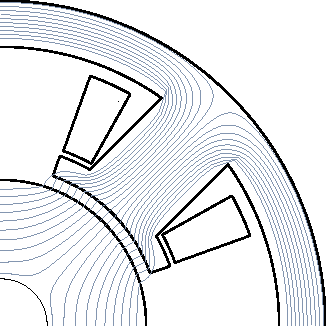
\includegraphics[width=0.4\textwidth]{fig/lec03/Ideal_air_gap_field.pdf}
				\caption{Idealized field lines (adapted from W.~Novender, \textit{Elektrische Maschinen}, Technische Hochschule Mittelhessen, 2023)}
				\label{fig:Ideal_air_gap_field}
			\end{figure}
		\end{column}
		\hfill
		\begin{column}{0.33\textwidth}
			\onslide<2->{\begin{figure}
				\centering
				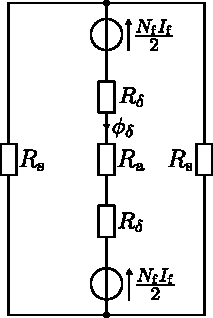
\includegraphics[height=0.65\textheight]{fig/lec03/Simplified_magnetic_network_DC_machine.pdf}
				\caption{Simplified magnetic network of a DC machine}
				\label{fig:Simplified_magnetic_network_DC_machine}
			\end{figure}}%
		\end{column}
	\end{columns}
\end{frame}

%%%%%%%%%%%%%%%%%%%%%%%%%%%%%%%%%%%%%%%%%%%%%%%%%%%%%%%%%%%%%
%% Air gap field (cont.) %%
%%%%%%%%%%%%%%%%%%%%%%%%%%%%%%%%%%%%%%%%%%%%%%%%%%%%%%%%%%%%%
\begin{frame}
	\frametitle{Air gap field (cont.)}
	\begin{columns}
		\begin{column}{0.65\textwidth}
			We introduce the following magnetic reluctances
			\begin{equation}
				\begin{alignedat}{2}
					R_\mathrm{s} &= \frac{l_\mathrm{s}}{\mu_{\mathrm{r, Fe}} \mu_0  A_\mathrm{s}} \quad  &&(\mbox{stator reluctance}), \\ \quad R_\mathrm{a} &= \frac{l_\mathrm{a}}{\mu_{\mathrm{r, Fe}}\mu_0  A_\mathrm{a}} \quad  &&(\mbox{armature reluctance}), \\
					R_\delta &= \frac{\delta}{\mu_0 A_\delta} \quad  &&(\mbox{air gap reluctance}).
				\end{alignedat}
			\end{equation}
			Above $l_i$ and $A_i$ are the respective lengths and cross-sectional areas of the field paths while $\delta$ is the air gap width. \onslide<2->{Furthermore, we have 
			$$ \mu_{\mathrm{r},\delta} = 1, \qquad \mu_{\mathrm{r, Fe}} >> 1 .$$}%
		\end{column}
		\hfill
		\begin{column}{0.35\textwidth}
			\begin{figure}
				\centering
				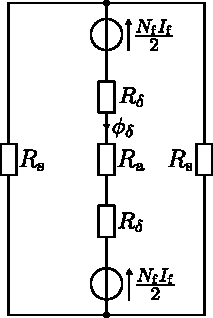
\includegraphics[height=0.65\textheight]{fig/lec03/Simplified_magnetic_network_DC_machine.pdf}
			\end{figure}
		\end{column}
	\end{columns}
\end{frame}

%%%%%%%%%%%%%%%%%%%%%%%%%%%%%%%%%%%%%%%%%%%%%%%%%%%%%%%%%%%%%
%% Air gap field (cont.) %%
%%%%%%%%%%%%%%%%%%%%%%%%%%%%%%%%%%%%%%%%%%%%%%%%%%%%%%%%%%%%%
\begin{frame}
	\frametitle{Air gap field (cont.)}
	\begin{columns}
		\begin{column}{0.65\textwidth}
			With $N_\mathrm{f}$ field winding turns and the field current $I_\mathrm{f}$, the air gap flux is given by:
			\begin{equation}
				\begin{split}
				\phi_\delta &= \frac{N_\mathrm{f} I_\mathrm{f}}{2 R_\delta + R_\mathrm{a} + \frac{1}{2}R_\mathrm{s}}\\
							& = \frac{N_\mathrm{f} I_\mathrm{f}}{\mu_0}\left(2\frac{\delta}{A_\delta} + \frac{l_\mathrm{a}}{\mu_{\mathrm{r, Fe}} A_\mathrm{a}} + \frac{1}{2}\frac{l_\mathrm{s}}{\mu_{\mathrm{r, Fe}} A_\mathrm{s}}\right)^{-1}. 
			\end{split}
			\label{eq:Air_gap_flux_DC_machine_simple}
			\end{equation}
			\onslide<2->{While the relative permeability of the iron paths is depending on the magnetic flux ($\mu_{\mathrm{r, Fe}} = \mu_{\mathrm{r, Fe}}(\phi)$) due to saturation (cf. \figref{fig:Permeability_of_ferromagnet}) rendering \eqref{eq:Air_gap_flux_DC_machine_simple} a nonlinear equation, we will assume that the air gap reluctance is dominating 
			\begin{equation}
				 R_\delta >> \left\{R_\mathrm{a}, R_\mathrm{s} \right\}
				 \label{eq:DC_flux_reluctance_simpl}
			\end{equation}}%
		\end{column}
		\hfill
		\begin{column}{0.35\textwidth}
			\begin{figure}
				\centering
				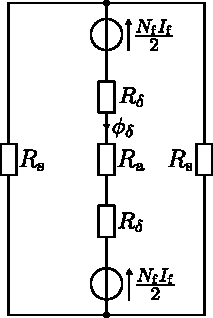
\includegraphics[height=0.65\textheight]{fig/lec03/Simplified_magnetic_network_DC_machine.pdf}
			\end{figure}
		\end{column}
	\end{columns}
\end{frame}

%%%%%%%%%%%%%%%%%%%%%%%%%%%%%%%%%%%%%%%%%%%%%%%%%%%%%%%%%%%%%
%% Air gap field (cont.) %%
%%%%%%%%%%%%%%%%%%%%%%%%%%%%%%%%%%%%%%%%%%%%%%%%%%%%%%%%%%%%%
\begin{frame}
	\frametitle{Air gap field (cont.)}
	Based on \eqref{eq:Air_gap_flux_DC_machine_simple} together with \eqref{eq:DC_flux_reluctance_simpl} we can simplify the effective air gap flux to
	\begin{equation}
		\phi_\delta = \frac{N_\mathrm{f} I_\mathrm{f}}{2 R_\delta} = \frac{N_\mathrm{F} I_\mathrm{f}}{2 \frac{\delta}{\mu_0 A_\delta}} = \frac{\mu_0 N_\mathrm{f} A_\delta}{2 \delta} I_\mathrm{f}.
		\label{eq:Air_gap_flux_DC_machine}
	\end{equation}\pause
	Here, $\delta$ is the air gap width and $A_\delta$ the effective cross-sectional area of the air gap which is
	\begin{equation}
		A_\delta = \alpha p \tau_\mathrm{p} l_z .
		\label{eq:Air_gap_area_DC_machine}
	\end{equation}\pause
	Above, the following assumptions and definitions are made:
	\begin{itemize}
		\item $l_z$ is the axial length of the machine. \pause
		\item The air gap width is very small such that the pole pitch $\tau_\mathrm{p}$ can be used as a good approximation for the air gap width in circumferential direction. \pause
		\item $\alpha$ is the pole coverage, that is, the ratio of the active pole surfaces to the pole pitch (cf. \figref{fig:Magnetic_field_normal_component_DC_machine} on next slide) representing the average field density in the air gap.
	\end{itemize}
\end{frame}

%%%%%%%%%%%%%%%%%%%%%%%%%%%%%%%%%%%%%%%%%%%%%%%%%%%%%%%%%%%%%
%% Air gap field (cont.) %%
%%%%%%%%%%%%%%%%%%%%%%%%%%%%%%%%%%%%%%%%%%%%%%%%%%%%%%%%%%%%%
\begin{frame}
	\frametitle{Air gap field (cont.)}
    \begin{figure}
        \centering
        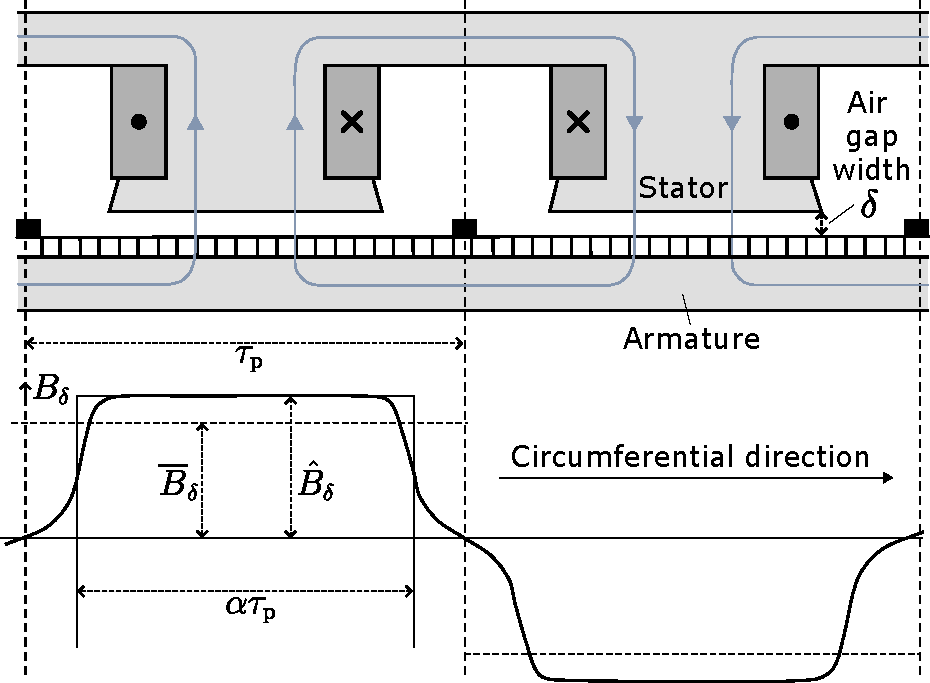
\includegraphics[height=0.67\textheight]{fig/lec03/Magnetic_field_normal_component_DC_machine.pdf}
        \caption{Principle magnetic field paths through stator and rotor as well as the (idealized) normal component of the magnetic field density $B_\delta$ in the air gap  (inspired from A. Binder, \textit{Elektrische Maschinen und Antriebe}, Vol. 2, Springer, 2017)}
		\label{fig:Magnetic_field_normal_component_DC_machine}
    \end{figure}
\end{frame}

%%%%%%%%%%%%%%%%%%%%%%%%%%%%%%%%%%%%%%%%%%%%%%%%%%%%%%%%%%%%%
%% Torque %%
%%%%%%%%%%%%%%%%%%%%%%%%%%%%%%%%%%%%%%%%%%%%%%%%%%%%%%%%%%%%%
\begin{frame}
	\frametitle{Torque}
    From \eqref{eq:Air_gap_flux_DC_machine} we can calculate the air gap flux density $B_\delta$ per pole pair as
	\begin{equation}
		B_\delta = \frac{\phi_\delta}{A_\delta} = \frac{\mu_0 N_\mathrm{f}}{2 \delta p} I_\mathrm{f}.
		\label{eq:Air_gap_flux_density_DC_machine}
	\end{equation}\pause
	The absolute Lorentz force per armature conductor is resulting in
	\begin{equation}
		F_\mathrm{c} =  B_\delta l_z I_\mathrm{c}= \frac{\mu_0 N_\mathrm{f} l_z}{4 \delta p a}I_\mathrm{f} I_\mathrm{a}.
		\label{eq:Lorentz_force_DC_machine_conductor}
	\end{equation}\pause
	Assuming that the air gap field lines are perpendicular to each armature conductor (cf. \figref{fig:Ideal_air_gap_field}), the torque per conductor for an armature diameter $d_\mathrm{a}$ is
	\begin{equation}
		T_\mathrm{c} = F_\mathrm{c} \frac{d_\mathrm{a}}{2} = \frac{\mu_0 N_\mathrm{f} l_z d_\mathrm{a}}{8 \delta p a} I_\mathrm{f} I_\mathrm{a}.
		\label{eq:Torque_DC_machine_conductor}
	\end{equation} \pause
	The resulting machine torque $T$ for $N_\mathrm{a}$ armature conductor loops from which an $\alpha$  share is covered by the poles (cf. \figref{fig:Magnetic_field_normal_component_DC_machine}) is
	\begin{equation}
		T = 2 \alpha N_\mathrm{a} T_\mathrm{c} = \frac{\mu_0 \alpha N_\mathrm{f} N_\mathrm{a} l_z d_\mathrm{a}}{4 \delta p a} I_\mathrm{f} I_\mathrm{a} .
		\label{eq:Torque_DC_machine}
	\end{equation}
\end{frame}